% ============================================================================
% Relatorio tecnico em duas colunas (estilo SBC), compilavel com pdflatex.
% Compilar:  latexmk -pdf relatorio.tex   (ou  pdflatex relatorio  duas vezes)
% Imagens necessarias (todas nesta mesma pasta):
%   segmentacao_exemplo.png, conv_eff_cong.png, conv_eff_ft.png,
%   conv_vgg_ft.png, cm_vgg_auto.png, cm_vgg_fixo.png
% ============================================================================
\documentclass[twocolumn,a4paper,11pt]{article}

\usepackage[utf8]{inputenc}
\usepackage[T1]{fontenc}
\usepackage{mathptmx}                 % Times (corpo)
\usepackage[scaled=0.9]{helvet}       % Helvetica (titulos)
\usepackage{courier}                  % monoespacada (codigo)
\usepackage[a4paper,margin=2cm,columnsep=0.7cm]{geometry}
\usepackage{graphicx,url,amsmath,booktabs,multirow,float}
\usepackage{caption,subcaption}
\usepackage{listings,xcolor}

% Rotulos em portugues (sem depender do babel)
\renewcommand{\figurename}{Figura}
\renewcommand{\tablename}{Tabela}
\renewcommand{\refname}{Referências}
\renewcommand{\abstractname}{Abstract}
\renewcommand{\lstlistingname}{Trecho}

\captionsetup{font=small,labelfont=bf}
\setlength{\parindent}{1.2em}
\setlength{\parskip}{0pt}

% Estilo dos trechos de codigo
\definecolor{cKw}{rgb}{0.10,0.10,0.65}
\definecolor{cCm}{rgb}{0.30,0.55,0.30}
\definecolor{cSt}{rgb}{0.60,0.20,0.20}
\definecolor{cBg}{rgb}{0.97,0.97,0.97}
\lstset{
  language=Python,
  basicstyle=\ttfamily\scriptsize,
  keywordstyle=\color{cKw}\bfseries,
  commentstyle=\color{cCm}\itshape,
  stringstyle=\color{cSt},
  backgroundcolor=\color{cBg},
  frame=single, rulecolor=\color{gray!40},
  breaklines=true, columns=fullflexible,
  showstringspaces=false, tabsize=2, aboveskip=4pt, belowskip=4pt,
}

% Layout: nao esticar colunas (evita vaos grandes) e nao hifenizar
% (os padroes de hifenizacao do portugues nao estao instalados neste ambiente;
%  sem eles a hifenizacao quebra silabas erradas, ex.: "fibrog-landular").
\raggedbottom
\hyphenpenalty=10000
\tolerance=2000
\emergencystretch=3em
\hbadness=10000

\title{}
\author{}
\date{}

\begin{document}

% ---------------------------------------------------------------------------
% Cabecalho, abstract e resumo ocupando a largura total da pagina
% ---------------------------------------------------------------------------
\twocolumn[{%
\centering
{\LARGE\bfseries Segmentação e Classificação da Densidade Mamária (BI\nobreakdash-RADS):\\[2pt]
um estudo comparativo entre base congelada e \emph{fine\nobreakdash-tuning} em VGG16 e EfficientNet\nobreakdash-B0\par}
\vspace{1.0em}
{\large Arthur Martinho Medeiros Oliveira\quad Luis Augusto Starling Toledo\quad Túlio Gomes Braga\par}
\vspace{0.5em}
{\normalsize Curso de Ciência da Computação, Pontifícia Universidade Católica de Minas Gerais (PUC Minas)\\
Campus Coração Eucarístico, Belo Horizonte, MG, Brasil\\
Disciplina de Processamento e Análise de Imagens, Prof. Alexei Manso Correa Machado\\
\texttt{813168}, \texttt{761670}, \texttt{802512} \texttt{@sga.pucminas.br}\par}
\vspace{1.4em}
\begin{minipage}{0.90\textwidth}
\small
\noindent\textbf{Abstract.}
This work presents a fully graphical application that segments the breast region in
mammograms and classifies breast density (BI\nobreakdash-RADS) using VGG16 and
EfficientNet\nobreakdash-B0, both pre\nobreakdash-trained on ImageNet. Segmentation combines CLAHE,
Otsu thresholding, largest connected component selection and region growing.
We systematically compare two transfer learning strategies (frozen base versus
fine\nobreakdash-tuning) and two class weighting schemes (automatic versus fixed), over the
binary and the four\nobreakdash-class tasks, totalling sixteen experiments. Fine\nobreakdash-tuning
clearly outperformed the frozen base on the four\nobreakdash-class task (VGG16: 0.577 to
0.712; EfficientNet\nobreakdash-B0: 0.564 to 0.692), while fixed weighting rebalanced the
confusion matrix, strongly improving the recall of the hardest class (II) with
little or no loss in overall accuracy.

\vspace{0.6em}
\noindent\textbf{Resumo.}
Este trabalho apresenta um aplicativo totalmente gráfico que segmenta a região da
mama e classifica a densidade mamária (BI\nobreakdash-RADS) com VGG16 e EfficientNet\nobreakdash-B0
pré\nobreakdash-treinadas na ImageNet. A segmentação combina CLAHE, limiarização de Otsu,
seleção da maior componente conexa e crescimento de regiões. Comparamos de forma
sistemática duas estratégias de \emph{transfer learning} (base congelada e
\emph{fine\nobreakdash-tuning}) e dois esquemas de ponderação de classes (automático e fixo),
nas tarefas binária e de quatro classes, totalizando dezesseis experimentos. O
\emph{fine\nobreakdash-tuning} superou nitidamente a base congelada nas quatro classes (VGG16:
0,577 para 0,712; EfficientNet\nobreakdash-B0: 0,564 para 0,692), e a ponderação fixa
reequilibrou a matriz de confusão, melhorando bastante a sensibilidade da classe
mais difícil (II) com pouca ou nenhuma perda de acurácia global.
\end{minipage}
\vspace{1.6em}
}]

% ---------------------------------------------------------------------------
\section{Introdução}

A densidade da mama está comprovadamente associada ao risco de câncer e à redução
da sensibilidade da mamografia, pois um tecido mais denso pode ocultar lesões. A
escala BI\nobreakdash-RADS, do \textit{American College of Radiology}, descreve essa densidade
em quatro níveis: quase inteiramente gordurosa (I), com tecido fibroglandular
difuso (II), denso heterogêneo (III) e extremamente denso (IV). Como a
classificação é feita por inspeção visual, ela sofre de variabilidade entre
observadores, o que motiva o uso de métodos automáticos de apoio à decisão.

Neste trabalho implementamos um aplicativo totalmente gráfico que lê e exibe
mamografias em PNG e TIFF com zoom, segmenta automaticamente a região da mama
(eliminando fundo e anotações), realiza aumento de dados por rotação, treina e
avalia as redes VGG16 e EfficientNet\nobreakdash-B0 nas tarefas binária e de quatro classes,
medindo métricas e tempos, e explica a decisão da rede com a técnica Grad\nobreakdash-CAM.
Para enriquecer a análise além do mínimo exigido, estruturamos o trabalho como um
estudo comparativo controlado: avaliamos duas estratégias de \emph{transfer
learning} (base congelada, como pede o enunciado, e \emph{fine\nobreakdash-tuning})
combinadas a dois esquemas de ponderação de classes, resultando em dezesseis
experimentos cujos resultados orientam as escolhas de projeto. A estratégia de
congelamento é escolhida na própria interface, por um seletor dedicado, e o mesmo
arquivo \texttt{main.py} executa as duas variantes.

% ---------------------------------------------------------------------------
\section{Materiais e Métodos}

\subsection{Conjunto de dados}

Utilizamos o conjunto \textbf{RMLO} (mama direita, incidência médio\nobreakdash-lateral
oblíqua), cujas quatro classes BI\nobreakdash-RADS correspondem às pastas \textbf{D, E, F, G}
(I, II, III e IV), com 314 imagens por classe. Conforme o enunciado, separamos para
teste as imagens cuja numeração é múltiplo de 4 e as demais para treino. Cada
classe contribui com 78 imagens de teste (múltiplos de 4 até 312) e 236 de treino.
Após a divisão, o treino reúne 944 imagens (4720 após o aumento por rotação) e o
teste 312, com 78 por classe. O conjunto de teste é, portanto, perfeitamente
balanceado, o que torna as comparações mais justas e faz a sensibilidade média
macro coincidir com a acurácia nas quatro classes.

\subsection{Segmentação}

A segmentação parte de uma premissa simples: a mama é a maior estrutura clara e
conexa da imagem, enquanto o fundo é escuro e as anotações (etiquetas e
marcadores) são objetos claros, porém pequenos e desconectados do tecido. A função
\texttt{segmentar\_mama} encadeia os seguintes passos: zeragem do canto
superior\nobreakdash-esquerdo (região típica da etiqueta); redução do maior lado da imagem
para 1024 pixels, de forma adaptativa ao tamanho original; zeragem das bordas;
filtro de mediana; realce local de contraste por \textbf{CLAHE} (\textit{clip}
2,0, blocos 8$\times$8); limiarização automática de \textbf{Otsu}; abertura
morfológica 5$\times$5; seleção da \textbf{maior componente conexa}, passo que
descarta as anotações; \textbf{crescimento de regiões} para alcançar o tecido
gorduroso periférico; fechamento morfológico; preenchimento de buracos por
\textit{flood fill}; e, por fim, a aplicação da máscara, que zera fundo e
anotações. Como os elementos estruturantes são dimensionados em proporção ao
tamanho da imagem, o método é praticamente invariante à resolução. A
Figura~\ref{fig:seg} mostra um resultado: a etiqueta textual no canto superior
desaparece na imagem segmentada, restando apenas a mama.

\begin{figure}[t]
\centering
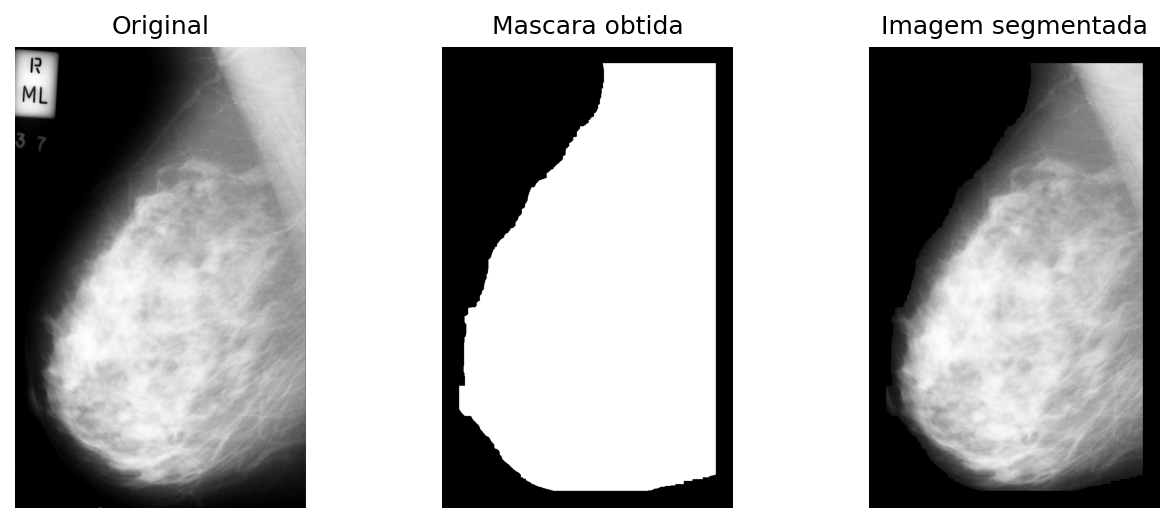
\includegraphics[width=0.92\linewidth]{segmentacao_exemplo.png}
\caption{Segmentação de um caso BI\nobreakdash-RADS IV: imagem original, máscara obtida e
imagem segmentada. A etiqueta e os marcadores do canto são removidos.}
\label{fig:seg}
\end{figure}

Os dois passos centrais, que diferenciam a solução de uma simples limiarização,
são a seleção da maior componente conexa (que isola a mama e descarta anotações) e
o crescimento de regiões controlado pelo limiar de Otsu, que recupera o tecido
gorduroso periférico sem invadir o fundo. O Trecho~\ref{lst:seg} resume esse
núcleo.

\noindent\begin{minipage}{\linewidth}
\begin{lstlisting}[caption={Núcleo da segmentação: maior componente conexa e crescimento de regiões.},label=lst:seg]
# maior componente conexa apos Otsu
n, rotulada, est, _ = cv2.connectedComponentsWithStats(aberta)
maior = 1 + int(np.argmax(est[1:, cv2.CC_STAT_AREA]))
mascara = np.where(rotulada == maior, 255, 0).astype(np.uint8)

# crescimento de regiao ate o tecido periferico
limiar = max(10, int(limiar_otsu * 0.60))
candidato = cv2.threshold(realcada, limiar, 255,
                          cv2.THRESH_BINARY)[1]
crescida = mascara.copy()
for _ in range(15):
    exp = cv2.dilate(crescida, np.ones((9, 9), np.uint8))
    exp = cv2.bitwise_and(exp, candidato)
    if np.array_equal(exp, crescida):
        break
    crescida = exp
\end{lstlisting}
\end{minipage}

\subsection{Aumento de dados}

Cada imagem de treino origina cinco variações rotacionadas em $-20$, $-10$, $0$,
$10$ e $20$ graus, com as bordas preenchidas em preto. Essas pequenas rotações
imitam variações reais de posicionamento da mama no exame, ampliam a base e ajudam
a reduzir o sobreajuste, sem introduzir distorções anatômicas que não ocorreriam na
prática. O aumento é aplicado apenas ao treino; validação e teste usam as imagens
originais.

\subsection{Classificadores e estratégias de \emph{transfer learning}}

Ambas as redes foram pré\nobreakdash-treinadas na ImageNet e recebem entrada RGB de
224$\times$224 (o tom de cinza é replicado nos três canais), normalizada pela média
e pelo desvio da ImageNet, condição para reaproveitar corretamente os pesos.
Comparamos duas estratégias de adaptação, selecionáveis na interface pelo seletor
\textit{Congelamento}:

\begin{itemize}
\item \textbf{Base congelada}: congela\nobreakdash-se a base convolucional e treina\nobreakdash-se
somente a parte completamente conectada, como pede o enunciado. O otimizador é o
Adam com taxa única ($10^{-3}$) e \emph{weight decay} de $10^{-4}$.
\item \textbf{Fine\nobreakdash-tuning}: a base também é treinada, mas com \textbf{taxas
discriminativas}, recebendo taxa menor ($10^{-4}$), enquanto a cabeça recebe taxa
maior ($10^{-3}$). A ideia é refinar a base sem destruir as \emph{features} já
aprendidas.
\end{itemize}

A Figura~\ref{fig:topo} resume a topologia. A VGG16 mantém o classificador denso
original, trocando a última camada por \texttt{Linear(4096, n)}; a
EfficientNet\nobreakdash-B0 usa \texttt{Dropout} seguido de \texttt{Linear(1280, n)}, com $n
\in \{2,4\}$. O Trecho~\ref{lst:cong} mostra como o seletor de congelamento define o
otimizador.

\begin{figure}[t]
\centering
\footnotesize
\setlength{\fboxsep}{5pt}
\fbox{Entrada $224\times224\times3$}\\[3pt]
$\downarrow$\\[3pt]
\fbox{Base convolucional (congelada ou $lr\cdot0{,}1$)}\\[3pt]
$\downarrow$\\[3pt]
\fbox{Cabeça densa, completamente conectada ($lr$)}\\[3pt]
$\downarrow$\\[3pt]
\fbox{Softmax (2 ou 4 classes)}
\caption{Topologia. Na base congelada apenas a cabeça treina; no
\emph{fine\nobreakdash-tuning} a base treina com taxa dez vezes menor que a da cabeça.}
\label{fig:topo}
\end{figure}

\noindent\begin{minipage}{\linewidth}
\begin{lstlisting}[caption={Seletor de congelamento e taxas discriminativas no laço de treino.},label=lst:cong]
if congelar:            # base congelada: so a cabeca
    p = [x for x in modelo.parameters()
         if x.requires_grad]
    otim = optim.Adam(p, lr=lr, weight_decay=1e-4)
else:                   # fine-tuning: taxas distintas
    otim = optim.Adam([
      {"params": modelo.features.parameters(),
       "lr": lr * 0.1},
      {"params": modelo.classifier.parameters(),
       "lr": lr}])
agend = optim.lr_scheduler.ReduceLROnPlateau(
    otim, mode="min", factor=0.5, patience=3)
\end{lstlisting}
\end{minipage}

\subsection{Esquemas de ponderação de classes}

Na função de perda (\texttt{CrossEntropyLoss}) comparamos dois esquemas de peso por
classe. No \textbf{automático}, o peso de cada classe é o inverso de sua frequência
no treino. No \textbf{fixo}, os pesos são definidos manualmente, $[1,1]$ na binária
e $[1,\,2,\,2,\,1{,}5]$ nas quatro classes, de modo a reforçar as classes II e III,
que são as mais difíceis. Como o conjunto é balanceado, o peso fixo não corrige
desbalanceamento; ele expressa uma prioridade clínica deliberada.

\subsection{Bibliotecas, funções e hiperparâmetros}

As bibliotecas utilizadas foram \textbf{OpenCV} (leitura de imagens, CLAHE, Otsu,
morfologia, componentes conexas e rotações), \textbf{PyTorch} com torchvision
(redes pré\nobreakdash-treinadas, treino e Grad\nobreakdash-CAM), \textbf{NumPy} (cálculo das
métricas), \textbf{Matplotlib} (gráficos) e \textbf{Tkinter} (interface gráfica). A
lógica de segmentação, o laço de treino, o cálculo das métricas a partir da matriz
de confusão e o Grad\nobreakdash-CAM são código próprio; das bibliotecas usamos apenas funções
elementares, com parâmetros descritos na Tabela~\ref{tab:hiper}.

\begin{table*}[t]
\centering
\caption{Principais hiperparâmetros e justificativa das escolhas.}
\label{tab:hiper}
\small
\begin{tabular}{p{3.6cm}p{4.0cm}p{8.2cm}}
\toprule
\textbf{Hiperparâmetro} & \textbf{Valor} & \textbf{Justificativa} \\
\midrule
Entrada e normalização & 224$\times$224, estatísticas da ImageNet & Resolução nativa das redes; alinha a entrada ao pré\nobreakdash-treino. \\
Otimizador & Adam & Adaptativo e robusto, com pouca calibração de hiperparâmetros. \\
Taxas (\emph{fine\nobreakdash-tuning}) & base $10^{-4}$, cabeça $10^{-3}$ & Refina a base sem degradar; a cabeça nova aprende mais rápido. \\
Taxa (base congelada) & única, $10^{-3}$, \emph{wd} $10^{-4}$ & Apenas a cabeça é treinada; \emph{weight decay} regulariza. \\
Agendador & ReduceLROnPlateau (fator 0,5, paciência 3) & Reduz a taxa quando a validação estagna. \\
\emph{Early stopping} & paciência 5, restaura melhores pesos & Para cedo e controla o sobreajuste. \\
\emph{Dropout} & 0,5 (VGG16); 0,3 (EfficientNet) & Regularização; valores de projeto de cada rede. \\
\emph{Batch} e épocas & VGG16 32/25; EfficientNet 16/50 & Cabe nos 8\,GB da GPU; épocas como teto. \\
Validação & 15\% estratificada, semente 42 & Monitoramento representativo e reprodutível. \\
Aumento & 5 rotações de $-20$ a $20$ graus & Variações de posicionamento plausíveis no exame. \\
\bottomrule
\end{tabular}
\end{table*}

\subsection{Métricas}

As métricas são calculadas a partir da matriz de confusão: sensibilidade
$=\mathrm{VP}/(\mathrm{VP}+\mathrm{FN})$, especificidade
$=\mathrm{VN}/(\mathrm{VN}+\mathrm{FP})$, precisão
$=\mathrm{VP}/(\mathrm{VP}+\mathrm{FP})$, acurácia
$=(\mathrm{VP}+\mathrm{VN})/\mathrm{total}$ e $F_1$, a média harmônica de precisão e
sensibilidade. Para quatro classes reportamos as médias macro de sensibilidade e
especificidade, cada classe contra as demais.

% ---------------------------------------------------------------------------
\section{Resultados}

Foram executados 16 experimentos, combinando 2 redes, 2 estratégias de
\emph{transfer learning}, 2 esquemas de peso e 2 tarefas. As
Tabelas~\ref{tab:bin} e~\ref{tab:quatro} consolidam, respectivamente, a tarefa
binária e a de quatro classes; os valores em negrito destacam as melhores
acurácias de cada tarefa.

\begin{table*}[t]
\centering
\caption{Classificação binária (I+II versus III+IV) no conjunto de teste.}
\label{tab:bin}
\small
\begin{tabular}{lllcccccc}
\toprule
\textbf{Rede} & \textbf{Estratégia} & \textbf{Peso} & \textbf{Acur.} & \textbf{Sens.} & \textbf{Espec.} & \textbf{Prec.} & \textbf{$F_1$} & \textbf{T.\ treino (s)} \\
\midrule
EfficientNet\nobreakdash-B0 & congelada    & automático & 0,8173 & 0,8333 & 0,8013 & 0,8075 & 0,8202 & 186,3 \\
EfficientNet\nobreakdash-B0 & congelada    & fixo       & 0,8173 & 0,8205 & 0,8141 & 0,8153 & 0,8179 & 178,4 \\
EfficientNet\nobreakdash-B0 & fine\nobreakdash-tuning & automático & 0,8622 & 0,8205 & 0,9038 & 0,8951 & 0,8562 & 137,2 \\
EfficientNet\nobreakdash-B0 & fine\nobreakdash-tuning & fixo       & \textbf{0,8654} & 0,8269 & 0,9038 & 0,8958 & 0,8600 & 142,7 \\
VGG16          & congelada    & automático & 0,8365 & 0,8013 & 0,8718 & 0,8621 & 0,8306 & 219,9 \\
VGG16          & congelada    & fixo       & 0,8365 & 0,8013 & 0,8718 & 0,8621 & 0,8306 & 210,6 \\
VGG16          & fine\nobreakdash-tuning & automático & 0,8526 & 0,7821 & 0,9231 & 0,9104 & 0,8414 & 468,4 \\
VGG16          & fine\nobreakdash-tuning & fixo       & \textbf{0,8750} & 0,8910 & 0,8590 & 0,8634 & 0,8770 & 458,4 \\
\bottomrule
\end{tabular}
\end{table*}

\begin{table*}[t]
\centering
\caption{Classificação em quatro classes (I, II, III, IV) no conjunto de teste.}
\label{tab:quatro}
\small
\begin{tabular}{lllcccc}
\toprule
\textbf{Rede} & \textbf{Estratégia} & \textbf{Peso} & \textbf{Acur.} & \textbf{Sens.\ média} & \textbf{Espec.\ média} & \textbf{T.\ treino (s)} \\
\midrule
EfficientNet\nobreakdash-B0 & congelada    & automático & 0,5641 & 0,5641 & 0,8547 & 125,7 \\
EfficientNet\nobreakdash-B0 & congelada    & fixo       & 0,5609 & 0,5609 & 0,8536 & 112,0 \\
EfficientNet\nobreakdash-B0 & fine\nobreakdash-tuning & automático & 0,6923 & 0,6923 & 0,8974 & 137,0 \\
EfficientNet\nobreakdash-B0 & fine\nobreakdash-tuning & fixo       & 0,6699 & 0,6699 & 0,8900 & 143,0 \\
VGG16          & congelada    & automático & 0,5769 & 0,5769 & 0,8590 & 163,9 \\
VGG16          & congelada    & fixo       & 0,6186 & 0,6186 & 0,8729 & 184,1 \\
VGG16          & fine\nobreakdash-tuning & automático & \textbf{0,7115} & 0,7115 & 0,9038 & 344,9 \\
VGG16          & fine\nobreakdash-tuning & fixo       & \textbf{0,7115} & 0,7115 & 0,9038 & 391,7 \\
\bottomrule
\end{tabular}
\end{table*}

\subsection{Efeito do congelamento e do peso (quatro classes)}

A Tabela~\ref{tab:sens} detalha a sensibilidade por classe da VGG16 e revela dois
efeitos nítidos. Primeiro, o \emph{fine\nobreakdash-tuning} eleva a acurácia global ao
permitir que a rede aprenda características específicas do domínio. Segundo, a
ponderação fixa \textbf{reequilibra} as classes: a classe II, de longe a mais
difícil, parte de uma sensibilidade de apenas 0,179 (base congelada, peso
automático) e chega a 0,603 (\emph{fine\nobreakdash-tuning}, peso fixo). A Figura~\ref{fig:cm}
ilustra esse reequilíbrio nas matrizes de confusão da VGG16 com \emph{fine\nobreakdash-tuning}:
com peso fixo, a mesma acurácia (0,712) distribui melhor os acertos entre as
classes, recuperando casos da classe II.

\begin{table}[h]
\centering
\caption{Sensibilidade por classe, VGG16, quatro classes.}
\label{tab:sens}
\small
\begin{tabular}{llcccc}
\toprule
\textbf{Estratégia} & \textbf{Peso} & \textbf{I} & \textbf{II} & \textbf{III} & \textbf{IV} \\
\midrule
congelada    & autom. & 0,782 & 0,179 & 0,795 & 0,551 \\
congelada    & fixo   & 0,628 & 0,538 & 0,577 & 0,731 \\
fine\nobreakdash-tuning & autom. & 0,897 & 0,397 & 0,718 & 0,833 \\
fine\nobreakdash-tuning & fixo   & 0,756 & 0,603 & 0,808 & 0,680 \\
\bottomrule
\end{tabular}
\end{table}

\begin{figure}[h]
\centering
\begin{subfigure}{0.49\linewidth}\centering
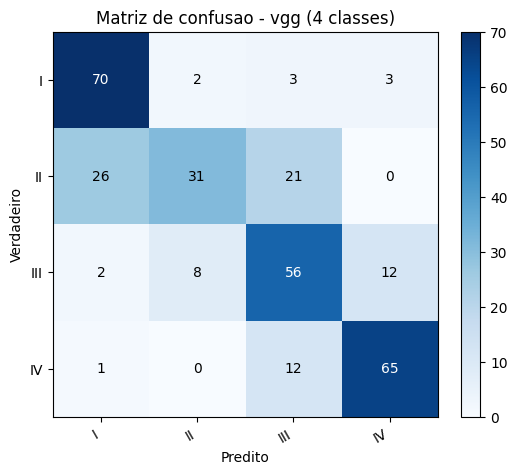
\includegraphics[width=\linewidth]{cm_vgg_auto.png}\\\footnotesize(a) Peso automático
\end{subfigure}\hfill
\begin{subfigure}{0.49\linewidth}\centering
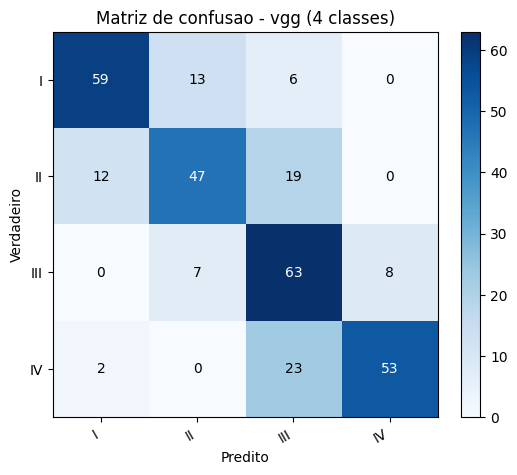
\includegraphics[width=\linewidth]{cm_vgg_fixo.png}\\\footnotesize(b) Peso fixo
\end{subfigure}
\caption{Matrizes de confusão da VGG16, quatro classes, \emph{fine\nobreakdash-tuning}. O peso
fixo melhora a classe II (de 31 para 47 acertos em 78), redistribuindo erros entre
classes vizinhas. Linha igual ao verdadeiro, coluna igual ao predito.}
\label{fig:cm}
\end{figure}

\subsection{Convergência e controle de sobreajuste}

A Figura~\ref{fig:conv} compara a convergência da EfficientNet\nobreakdash-B0 em quatro
classes. Com a base congelada (a), tanto a perda de treino quanto a de validação
estacionam em torno de 0,8 e a acurácia fica em torno de 0,63, sintoma clássico de
\emph{underfitting}, pois as \emph{features} da ImageNet não capturam plenamente a
textura de densidade. Com \emph{fine\nobreakdash-tuning} (b), a perda de treino cai bem mais e
a acurácia sobe.

\begin{figure}[h]
\centering
\begin{subfigure}{0.49\linewidth}\centering
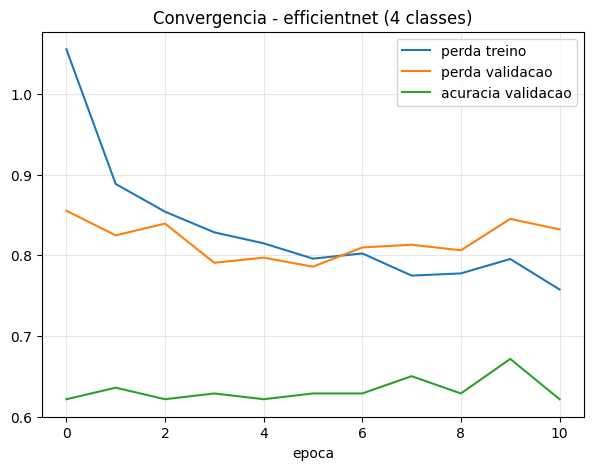
\includegraphics[width=\linewidth]{conv_eff_cong.png}\\\footnotesize(a) Base congelada
\end{subfigure}\hfill
\begin{subfigure}{0.49\linewidth}\centering
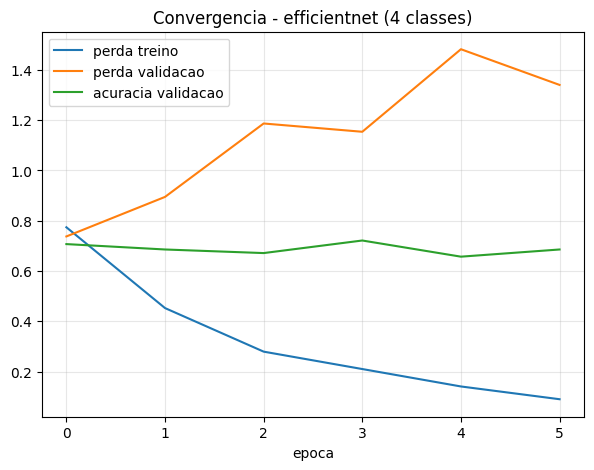
\includegraphics[width=\linewidth]{conv_eff_ft.png}\\\footnotesize(b) Fine\nobreakdash-tuning
\end{subfigure}
\caption{Convergência da EfficientNet\nobreakdash-B0, quatro classes, peso automático. A base
congelada estaciona (\emph{underfitting}); o \emph{fine\nobreakdash-tuning} reduz a perda de
treino e eleva a acurácia.}
\label{fig:conv}
\end{figure}

O reverso do \emph{fine\nobreakdash-tuning} aparece na VGG16 (Figura~\ref{fig:over}): a perda
de treino despenca para perto de zero enquanto a de validação cresce de forma
acentuada, indício de \emph{overfitting}. É exatamente aqui que o \emph{early
stopping} atua, restaurando os pesos da época de menor perda de validação. O log
real desse experimento (Trecho~\ref{lst:log}) torna o fenômeno explícito: a melhor
validação ocorre na época 1, e as épocas seguintes apenas memorizam o treino.

\begin{figure}[h]
\centering
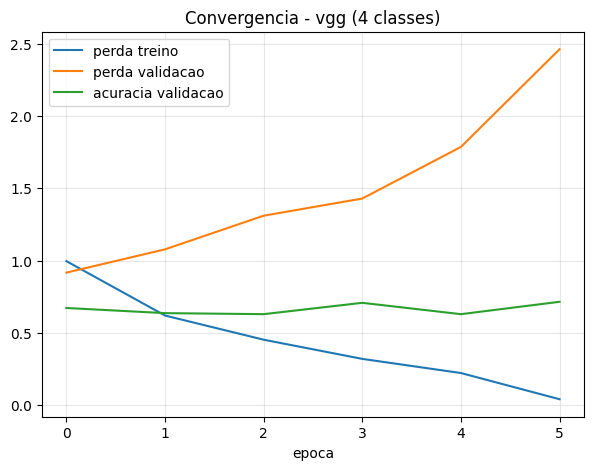
\includegraphics[width=0.74\linewidth]{conv_vgg_ft.png}
\caption{Convergência da VGG16, quatro classes, \emph{fine\nobreakdash-tuning}. A perda de
validação dispara enquanto a de treino cai: \emph{overfitting} contido pelo
\emph{early stopping}.}
\label{fig:over}
\end{figure}

\noindent\begin{minipage}{\linewidth}
\begin{lstlisting}[caption={Log real (VGG16, quatro classes, fine-tuning, peso automático).},label=lst:log]
# ep  treino   val      acc_val
  01  0.9959   0.9163   0.6714
  02  0.6191   1.0776   0.6357
  03  0.4516   1.3106   0.6286
  04  0.3188   1.4295   0.7071
  05  0.2208   1.7871   0.6286
  06  0.0394   2.4639   0.7143
# early stopping mantem a epoca 1 (menor val)
\end{lstlisting}
\end{minipage}

\subsection{Tempos de execução}

Todos os experimentos foram executados em uma GPU NVIDIA GeForce RTX 4060 (8\,GB). A
EfficientNet\nobreakdash-B0 treinou em aproximadamente 112 a 186 segundos por experimento,
enquanto a VGG16 levou de 164 a 468 segundos, de três a quatro vezes mais. A
inferência no conjunto de teste variou de cerca de 0,7 segundo (EfficientNet) a
cerca de 12 segundos (VGG16 binária), valor inflado na primeira avaliação porque
inclui a segmentação das imagens de teste enquanto o \emph{cache} ainda está vazio.

\subsection{Explicabilidade com Grad\nobreakdash-CAM}

A interface permite escolher uma imagem, classificá\nobreakdash-la e visualizar o mapa de
Grad\nobreakdash-CAM sobreposto. A técnica registra as ativações e os gradientes da última
camada convolucional, pondera os canais pela média espacial do gradiente da classe
predita e aplica uma ReLU, conforme o Trecho~\ref{lst:cam}. Nos casos analisados, a
ativação se concentra sobre o tecido fibroglandular, justamente a região que define
a densidade, o que indica que a rede decide por razões coerentes com o critério
clínico, e não por artefatos do fundo.

\noindent\begin{minipage}{\linewidth}
\begin{lstlisting}[caption={Núcleo do Grad-CAM: hooks e combinação ponderada.},label=lst:cam]
camada.register_forward_hook(guardar_ativacoes)
camada.register_full_backward_hook(guardar_grad)
...
saida = modelo(entrada)
saida[0, classe].backward()
w = gradientes.mean(dim=(2, 3), keepdim=True)
mapa = torch.relu((w * ativacoes).sum(dim=1))
\end{lstlisting}
\end{minipage}

\subsection{Ajuste de hiperparâmetros}

A Tabela~\ref{tab:ajuste} resume alternativas avaliadas no processo de ajuste e o
motivo de cada descarte. Chegamos ao conjunto final (Adam, ReduceLROnPlateau,
\emph{early stopping}, perda de entropia cruzada ponderada) por ser o mais simples
e defensável, mantendo a comparação controlada entre os dois esquemas de peso.

\begin{table}[h]
\centering
\caption{Resultados intermediários do ajuste de hiperparâmetros.}
\label{tab:ajuste}
\small
\begin{tabular}{p{2.5cm}p{5.1cm}}
\toprule
\textbf{Alternativa} & \textbf{Resultado e decisão} \\
\midrule
\emph{Batch} 128 & Estourou a memória da GPU sem ganho. Mantido 16/32. \\
Agendador cosseno & Decai de forma monotônica e conflita com o \emph{early stopping}. Trocado por ReduceLROnPlateau. \\
\emph{Focal loss} & Hiperparâmetro extra sem ganho no conjunto balanceado. Mantida a entropia cruzada ponderada. \\
\emph{Label smoothing} & Sem melhora clara; descartado. \\
Escala fixa 50\% na segmentação & Trocada por redução adaptativa do maior lado para 1024 px, mais robusta à resolução. \\
\bottomrule
\end{tabular}
\end{table}

% ---------------------------------------------------------------------------
\section{Discussão}

\textbf{Segmentação.} A combinação de Otsu, morfologia, maior componente conexa e
crescimento de regiões isolou a mama e removeu fundo e anotações na maioria dos
casos, como na Figura~\ref{fig:seg}. O crescimento de regiões foi importante para
incluir o tecido periférico, que também conta para a densidade. A principal
limitação ocorre quando uma anotação clara encosta na mama, situação em que a
seleção da maior componente pode não separá\nobreakdash-la; nesses casos a máscara tende a
incorporar a etiqueta.

\textbf{Por que a tarefa de quatro classes é mais difícil.} Na binária, agrupar
I+II contra III+IV coloca a fronteira de decisão na transição mais fácil, entre
mamas predominantemente gordurosas e predominantemente densas. Já as quatro classes
exigem distinguir níveis vizinhos de aparência contígua; a passagem de II
(fibroglandular difuso) para III (denso heterogêneo) é gradual e ambígua até para
radiologistas. As matrizes de confusão confirmam isso: os erros se concentram entre
classes adjacentes (II confundida com I e III) e quase nunca entre extremos (I com
IV). Por isso a acurácia cai de cerca de 0,87 na binária para cerca de 0,71 nas
quatro classes.

\textbf{Por que o \emph{fine\nobreakdash-tuning} superou a base congelada.} Com a base
congelada, a rede só recombina características aprendidas em imagens naturais, o que
resolve o contraste grosso (densa contra gordurosa), mas não a textura fina que
separa II de III, daí o \emph{underfitting} da Figura~\ref{fig:conv}(a). Ao
destravar a base e ajustá\nobreakdash-la ao domínio mamográfico com taxa baixa, a rede passa
a representar essa textura. Não por acaso o ganho é bem maior nas quatro classes
(cerca de 13 pontos) do que na binária (cerca de 2 a 5 pontos), que o conhecimento
genérico já resolvia. As taxas discriminativas foram decisivas: usar a mesma taxa
alta na base e na cabeça destruiria os pesos pré\nobreakdash-treinados antes de a cabeça
estabilizar.

\textbf{Por que o peso fixo reequilibra.} Os pesos multiplicam o custo de errar
cada classe. Com peso uniforme, a rede tende a abandonar a classe mais ambígua (II)
e apostar nas vizinhas, pois isso minimiza a perda média, daí a sensibilidade de
apenas 0,179 da classe II na VGG16 congelada. Ao dobrar o peso de II e III, esses
erros passam a custar mais, e a rede desloca as fronteiras para recuperá\nobreakdash-los, ao
preço de um leve recuo nas classes fáceis (I e IV). Como o conjunto é balanceado,
trata\nobreakdash-se de uma escolha de prioridade clínica, mantendo (VGG16 \emph{fine\nobreakdash-tuning})
ou até elevando (VGG16 congelada, de 0,577 para 0,619) a acurácia global.

\textbf{VGG16 contra EfficientNet\nobreakdash-B0.} A VGG16, com sua parte densa muito maior,
tem mais capacidade para se ajustar ao conjunto pequeno e atingiu o maior pico nas
quatro classes (0,712); em compensação, sofre \emph{overfitting} mais forte
(Figura~\ref{fig:over}) e custa de três a quatro vezes mais tempo. A
EfficientNet\nobreakdash-B0, projetada para eficiência, é mais rápida e estável, com acurácia
apenas um pouco menor (0,692). A escolha depende do objetivo: maior acerto absoluto
(VGG16) ou melhor custo\nobreakdash-benefício (EfficientNet\nobreakdash-B0).

\textbf{Exemplos de erros e acertos.} Os acertos mais sólidos estão nas classes
extremas (I e IV têm as maiores sensibilidades). O erro mais ilustrativo aparece na
VGG16 congelada com peso automático: das 78 imagens de classe II, apenas 14 foram
acertadas, com 30 confundidas com I e 34 com III, exatamente a fronteira ambígua.
Esse padrão melhora muito com peso fixo e \emph{fine\nobreakdash-tuning}, como mostra a
Figura~\ref{fig:cm}.

% ---------------------------------------------------------------------------
\section{Conclusão}

Implementamos um aplicativo gráfico completo para segmentação e classificação da
densidade mamária, avaliado em 16 experimentos. O \emph{fine\nobreakdash-tuning} superou a
base congelada de forma consistente, com a VGG16 atingindo 0,712 nas quatro classes
e a EfficientNet\nobreakdash-B0 atingindo 0,865 na binária, confirmando que adaptar a base ao
domínio reduz o \emph{underfitting} herdado do pré\nobreakdash-treino em imagens naturais. A
comparação de esquemas de peso mostrou que a ponderação fixa reequilibra as
classes, beneficiando a classe mais difícil (II) sem perda relevante de acurácia.
Como trabalhos futuros, destacam\nobreakdash-se o \emph{fine\nobreakdash-tuning} parcial, descongelando
apenas as últimas camadas, mais adequado a conjuntos pequenos, e a busca
sistemática de pesos por classe.

% ---------------------------------------------------------------------------
\begin{thebibliography}{9}
\small
\bibitem{simonyan2015} SIMONYAN, K.; ZISSERMAN, A. Very Deep Convolutional Networks
for Large\nobreakdash-Scale Image Recognition. In: \textit{ICLR}, 2015.
\bibitem{tan2019} TAN, M.; LE, Q. EfficientNet: Rethinking Model Scaling for
Convolutional Neural Networks. In: \textit{ICML}, 2019.
\bibitem{selvaraju2017} SELVARAJU, R. R. et al. Grad\nobreakdash-CAM: Visual Explanations from
Deep Networks via Gradient\nobreakdash-based Localization. In: \textit{ICCV}, 2017.
\bibitem{otsu1979} OTSU, N. A Threshold Selection Method from Gray\nobreakdash-Level
Histograms. \textit{IEEE TSMC}, 1979.
\end{thebibliography}

\end{document}
